%% This is file `DEMO-TUDaSciPoster.tex' version 3.23 (2022/03/21),
%% it is part of
%% TUDa-CI -- Corporate Design for TU Darmstadt
%%
% !TeX program = lualatex
%%

\documentclass[
	accentcolor=3c,
%	boxstyle= boxed, % Boxen mit abgerundeten Ecken, farbigem Titelblock
	boxstyle=colored % Boxen mit farbigen Titelblock, keine vertikalen Linien
%	boxstyle=default % Voreinstellung, ohne Farbe, ohne vertikale Linien
%	logofile=example-image, %Falls die Logo Dateien nicht vorliegen
	]{tudasciposter}

%Sprache
\usepackage[ngerman,main=english]{babel}
\usepackage[autostyle]{csquotes}


\usepackage{multicol}
\usepackage{booktabs}
\usepackage{tabularx}
\usepackage[version=4,arrows=pgf-filled]{mhchem}

\def\app#1#2{%
	\mathrel{%
		\setbox0=\hbox{$#1\sim$}%
		\setbox2=\hbox{%
			\rlap{\hbox{$#1\propto$}}%
			\lower1.1\ht0\box0%
		}%
		\raise0.25\ht2\box2%
	}%
}
\def\approxprop{\mathpalette\app\relax}


\begin{document}
	\title{Two-layered Vectorial Kernel Models for Detailed Surface Kinetics using a Goal-Oriented Approach}
	\author{\underline{Felix Döppel}\inst{1,*} Tizian Wenzel\inst{2} \and Robin Herkert\inst{2} \and Bernard Haasdonk\inst{2} \and Martin Votsmeier\inst{1,3}}
	\institute{\inst{1}Technische Universität Darmstadt,  64287 Darmstadt, Germany, \hfill \inst{*}Contact: felix.doeppel@tu-darmstadt.de \\
	\inst{2}Universität Stuttgart, 70511 Stuttgart, Germany, \\
	\inst{3}Umicore AG \& Co. KG, 63457 Hanau, Germany
	}
	%\inst kann in den Autor und Institutsfeldern genutzt werden um eine Zuordnung zu ermöglichen. Bei Nummerierung ist der Nutzer dafür verantwortlich Konflikte mit \thanks zu vermeiden.
	%\titlegraphic{\includegraphics[width=.5\linewidth]{example-image}}
%	\footerqrcode{https://www.chemie.tu-darmstadt.de/votsmeier/ak_votsmeier/index.en.jsp}
	\footerqrcode{https://doi.org/10.26434/chemrxiv-2022-qjcs5}
	\footer{
		[1] D. Micale, C. Ferroni, R. Uglietti, M. Bracconi, M. Maestri, \textit{Chemie-Ingenieur-Technik} \textbf{2022}, 1–19. \newline
		[2] A. B. Mhadeshwar, D. G. Vlachos, \textit{J. Phys. Chem. B} \textbf{2004}, \textit{108}, 15246–15258.\newline
%		[3] S. Matera, M. Maestri, A. Cuoci, K. Reuter, \textit{ACS Catal.} \textbf{2014}, \textit{4}, 4081–4092.\newline
		[3] F. A. Döppel, M. Votsmeier, \textit{Chemrxiv} \textbf{2022}, DOI 10.26434/chemrxiv-2022-qjcs5.\newline
		Graphical abstract has been designed using resources from Flaticon.com
	}

%Instituts/Sponsorenlogos von links nach rechts
\footergraphics{
	\includegraphics[height=\height]{abb/Profile_Pic_FD}
}

\begin{tcbposter}[
	poster={
		columns=8,
		rows=12,
		spacing=1cm,
%		showframe, %Gitter einblenden. Für Platzierung häufig hilfreich
	},]

\begin{posterboxenv}[title=1. Introduction]{name=intro,column=1,row=5,span=4,rowspan=2}
	\vspace{-1.6cm} %dirty hack for more space
	\begin{itemize}
		\item \textbf{Detailed multi-scale modeling} provides valuable insights
		\item Kinetics are \textbf{computational bottleneck}\textsuperscript{[1]}
		\item Machine Learning surrogates speed up simulations
		\item Challenge: established schemes don't work if rate changes sign
	\end{itemize}
\end{posterboxenv}

\begin{posterboxenv}{name=GraphicalAbstract,column=1,row=1,span=8,rowspan=4}
	\centering
	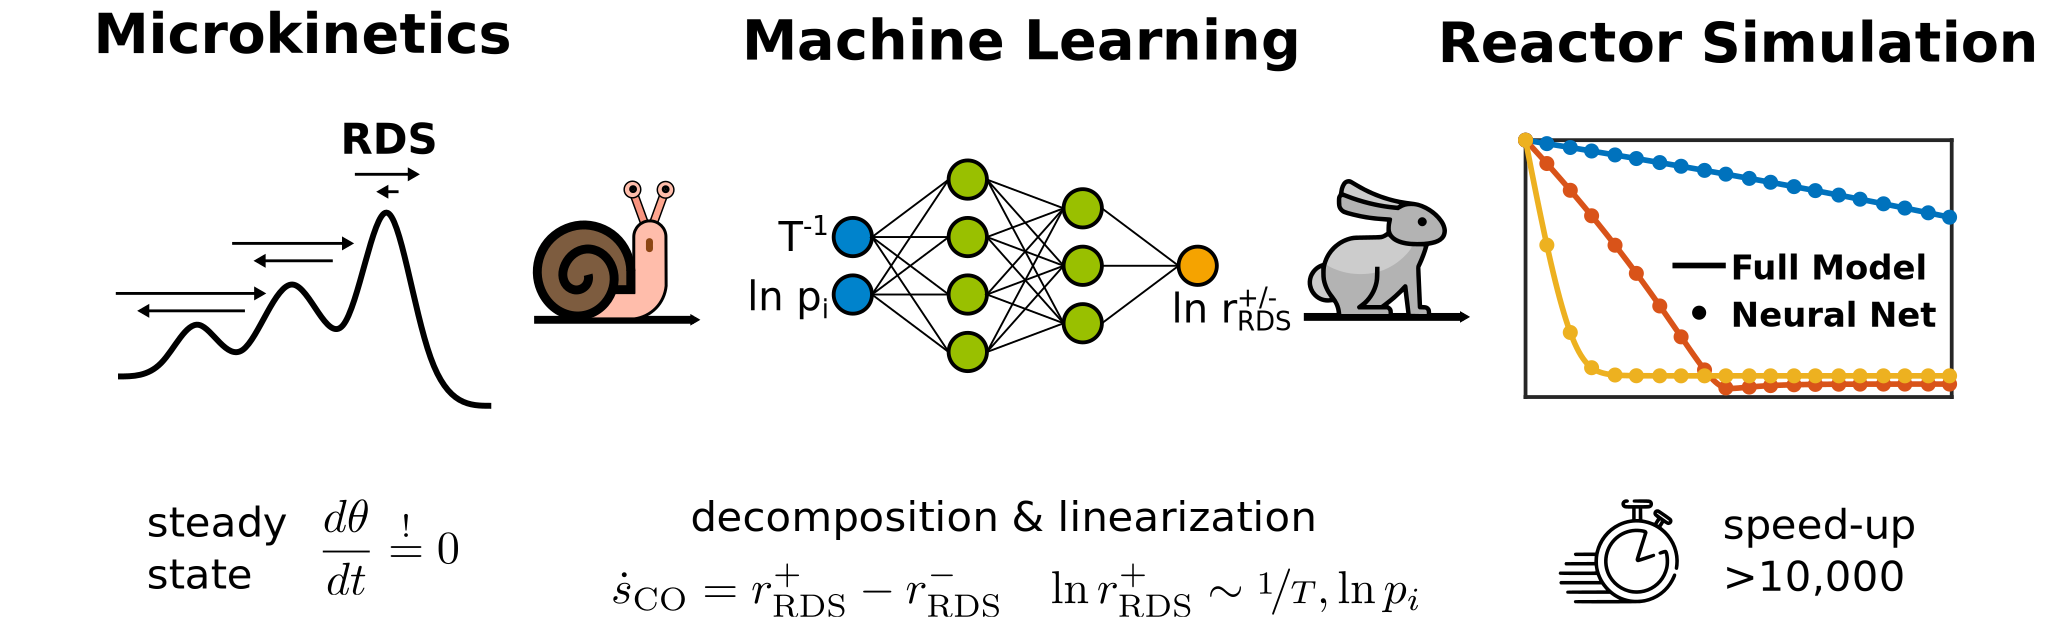
\includegraphics[width=\linewidth]{abb/Graphical_Abstract_alternative_fine}
\end{posterboxenv}

\begin{posterboxenv}[title=2. Methods]{name=Methods,column=5,row=5,span=4,rowspan=2}
	\vspace{-1.6cm} %dirty hack for more space
	\begin{itemize}
		\item Solve PrOx mechanism for steady state\textsuperscript{[2]}  %\textsuperscript{1}
		\item Find suitable reaction sets with reaction path analysis		
		\item Separately model $r_\text{forward}$ and $r_\text{reverse}$	
		\item Validate in plug-flow reactor simulation
	\end{itemize}

\end{posterboxenv}

\begin{posterboxenv}{name=RPA,row=7,rowspan=4,column=5,span=4}
	
\includegraphics[width=\linewidth]{abb/Fig_4_extended_fine_thick}
	\captionof{figure}{Suitable reaction sets can be identified with the reaction path. Using these sets for the prediction of \ce{CO} source terms, the prediction error correlates with the reversibility of the reactions. The rate-determining steps perform best.}
\end{posterboxenv}
%\draw[accentcolor,line width=4pt,->] ([yshift=0cm]TCBPOSTER@Methods.west) -|  ([xshift=-0.5cm]TCBPOSTER@RPA.west) -- (TCBPOSTER@RPA.west);
\begin{posterboxenv}[title=3. Results]{name=Results,column=1,row=7,span=4,rowspan=4}
	\vspace{-1.6cm} %dirty hack for more space
	\begin{itemize}
		\item Prediction error correlates with reversibility
		\item Using rate-determining step \textbf{increases accuracy by factor >100}
		\item Linearization allows for \textbf{lightweight models}
		\item Neural Networks outperform splines regarding accuracy, storage, \\ speed \& required data
		\item Concentration profile in plug-flow reactor simulation is reproduced \\with insignificant error	
	\end{itemize}
	\centering
	
\includegraphics[width=.75\linewidth]{abb/nngtspline}
\end{posterboxenv}

\begin{posterboxenv}[title=4. Conclusion]{name=Conclusion,column=1,row=11,span=8,rowspan=2}
\begin{multicols}{2}		
	\begin{itemize}
		\item Machine Learning surrogates speed up detailed multi-scale simulations
		\item Decomposing source terms into rate-determining reactions is key%yields efficient surrogates
		\item Method can be paired with any regression model (NN, RF, SVM, $\dots$)
		\item \textbf{Scalability towards complex mechanisms} like kinetic Monte-Carlo
		\item First step towards \textbf{learning from data directly}
		\item Details are available as preprint\textsuperscript{[3]} (scan QR-code)
	\end{itemize}
\end{multicols}

\end{posterboxenv}

\end{tcbposter}

\end{document}


